
\documentclass[11pt]{article}
\usepackage[portuges]{babel}
\usepackage[utf8]{inputenc}
\usepackage{graphicx}
\usepackage[hidelinks]{hyperref}
\usepackage[toc,page]{appendix}
\usepackage{placeins}
\usepackage{float}
\usepackage{indentfirst}

\renewcommand\appendixtocname{Anexos}
\renewcommand\appendixpagename{Anexos}

\begin{document}
\sloppy

\begin{titlepage}

% Defines a new command for the horizontal lines, change thickness here
\newcommand{\HRule}{\rule{\linewidth}{0.5mm}}

\center % Center everything on the page
 
% HEADING SECTIONS
\textsc{\LARGE Engenharia de Segurança}\\[1.5cm]
\textsc{\Large Universidade do Minho}\\[0.5cm]
\textsc{\large Mestrado Integrado em Engenharia Informática}\\[0.6cm]

% TITLE SECTION
\vspace{0.8cm}
\HRule \\[0.6cm]
{ \huge \bfseries Projeto em Identificação \textit{mobile}}\\[0.4cm]
{ \Large \bfseries \textbf{mDL} (\textit{mobile Driving License})} \\[0.4cm]
\HRule \\[1.2cm]

% AUTHOR SECTION
\Large \emph{Autores:}\\
A77531 - Daniel Maia\\
A78034 - Diogo Costa\\
A77364 - Mafalda Nunes\\[1.3cm]

% DATE SECTION
{\large \today}\\[1.5cm]

% LOGO SECTION

\includegraphics[width=0.55\textwidth]{logo}\\[1cm]

\vfill % Fill the rest of the page with whitespace

\end{titlepage}


\begin{abstract}
% TODO: Resumo
\end{abstract}

\vspace{0.8cm}

\tableofcontents

\newpage

\hypersetup{
	colorlinks=false,
	allbordercolors={0 0 0},
	pdfborderstyle={/S/U/W 1}
}


\section{Introdução}

Este projeto é desenvolvido no âmbito da unidade curricular de Engenharia de Segurança, do Mestrado Integrado em Engenharia Informática, da Universidade do Minho.

Um dos principais objetivos deste trabalho é a investigação e análise do \textit{standard} ISO de desmaterialização da Carta de Condução, mais especificamente o ``\texttt{ISO/IEC CD 18013-5 Information technology} -- \texttt{Personal identification} -- \texttt{ISO compliant driving licence} -- \texttt{Part 5: Mobile driving licence application (mDL)}''. Pretende-se dar especial atenção à estrutura de dados requerida e aos vários algoritmos, primitivas criptográficas e \textit{workflows} que garantem a segurança da mDL. Por fim, deverá apresentar-se uma implementação da mDL, de acordo com o ISO, através da utilização de bibliotecas \textit{open-source}.

De facto, esta desmaterialização de documentos, que se baseia em técnicas e algoritmos criptográficos, torna possível o acesso aos mesmos através de dispositivos móveis, que são comummente utilizados na atualidade. Assim, começa a surgir a tendência de substituir os documentos de identificação, como hoje os conhecemos (em papel ou \textit{smartcard}), por documentos desmaterializados.


\section{Contextualização}

O \textit{standard} ISO/IEC (\textit{International Organization for Standardization} / \textit{International Electrotechnical Commission}) 18013 é caracterizado pelo titulo geral \texttt{Personal Identification — ISO
Compliant Driving Licence} e consiste nas seguintes partes:

\begin{itemize}
	\item \textbf{Parte 1} -- \texttt{Physical Characteristics and Basic Data Set}: descreve as características físicas, o conjunto de elementos de dados básico, o \textit{layout} visual e capacidades de segurança físicas (recursos legíveis pelo ser humano) de uma \textit{ISO-compliant driving licence} (IDL);
	\item \textbf{Parte 2} -- \texttt{Machine-Readable Technologies}: descreve as tecnologias, legíveis por máquina, que podem ser utilizadas por este \textit{standard}, incluindo a estrutura de dados lógica e o mapeamento de dados por cada tecnologia;
	\item \textbf{Parte 3} -- \texttt{Access Control, Authentication and Integrity Validation}: descreve as capacidades de segurança eletrónica que podem incorporar este \textit{standard}, incluindo mecanismos para controlo de acesso aos dados, verificação da origem de uma IDL e confirmação da integridade dos dados;
	\item \textbf{Parte 4} -- \texttt{Test Methods}: descreve métodos de teste que podem ser utilizados para determinar se uma IDL está de acordo com os requisitos das tecnologias legíveis por máquinas especificadas na parte 2 e com as capacidades de segurança eletrónica especificadas na parte 3.
\end{itemize}

Este \textit{standard} cria uma base comum para a utilização internacional e reconhecimento mútuo da IDL, sem impedir que países ou estados apliquem as suas regras de privacidade e que autoridades nacionais/comunitárias/regionais de trânsito tratem das suas necessidades específicas.

Assim, estas partes do ISO/IEC 18013 permitem estandardizar uma carta de condução eletrónica, com um cartão *chip* com ou sem contacto. É utilizada tecnologia derivada do passaporte eletrónico e exemplos de mecanismos de segurança utilizados para controlo de acesso são BAP (\textit{Broadcast Authentication Using Cryptographic Puzzles}), SAC/PACE (\textit{Supplemental Access Control} / \textit{Password Authenticated Connection Establishment}) e EAP (\textit{Extensible Authentication Protocol}).

A \textbf{Parte 5} do ISO/IEC 18013 -- \texttt{Mobile Driving Licence} -- pretende estabelecer um \textit{standard} para especificações de interface para a implementação de cartas de condução associadas a dispositivos móveis (\textit{Mobile Driving License} - mDL), isto é, dispositivos eletrónicos com interface de utilizador, a capacidade de armazenar informação da mDL e de a partilhar com um leitor, após instrução do titular (\textit{smartphones}, \textit{wearables}, entre outros). Um leitor mDL é um dispositivo portátil ou computador, que pode trocar dados com uma mDL, enquanto que o titular da mDL é o indivíduo para quem a mDL é emitida, isto é, o titular legítimo dos privilégios de condução refletidos na mDL.

Esta parte do ISO/IEC 18013 descreve a interface e requisitos físicos e funcionais associados que possibilitam a utilização de dispositivos móveis pelo titular da carta de condução, para a fornecer a um verificador, facilitando o acesso do mesmo a informação da carta de condução.

O objetivo é permitir que verificadores não associados à autoridade de emissão da mDL, como outras autoridades de emissão ou entidades verificadoras de outros países, ganhem acesso à informação para a qual o titular da mDL providenciar consentimento, conseguindo autenticá-la. Para o conjunto de informações disponibilizado pelo titular da mDL, estas entidades deverão poder:

\begin{enumerate}
	\item Utilizar uma máquina para obter a informação da mDL;
	\item Estabelecer a conexão entre a mDL e o seu titular com um grau aceitável de confiança;
	\item Autenticar a origem da informação mDL;
	\item Verificar a integridade da informação mDL.
\end{enumerate}

Outra vantagem das mDL em relação às cartas de condução físicas é a capacidade de atualizar informação com mais frequência e autenticá-la com um nível de confiança superior.

Existem três interfaces fulcrais para esta parte do *standard*, que são explicadas de seguida:

\begin{enumerate}
	\item Interface entre a mDL e a autoridade emissora, que permite controlar, entre outros, como o mDL é fornecido e como são efetuadas atualizações. Esta interface não é o foco desta parte do ISO/IEC 18013, uma vez que a interoperabilidade entre autoridades emissoras não é requerida para as funcionalidades pretendidas.
	\item Interface entre a mDL e o leitor, que tem de funcionar em tempo real e é descrita nesta parte do ISO/IEC 18013.
	\item Interface entre a autoridade emissora e a entidade de verificação, que facilita a troca de informação requerida para permitir a um leitor confirmar a autenticidade da informação da mDL e, em alguns casos, ler alguma informação da mesma. Esta interface é estabelecida preferencialmente entre a entidade verificadora e a autoridade emissora (diretamente ou através de intermediários), em vez de diretamente entre o leitor e a autoridade de emissão. Para além disso, não precisa de funcionar em tempo real e pode ser usada pela própria autoridade emissora, em leitores sob o seu controlo. Esta interface será descrita nesta parte do ISO/IEC 18013.
\end{enumerate}

\begin{figure}[H]
	\centering
	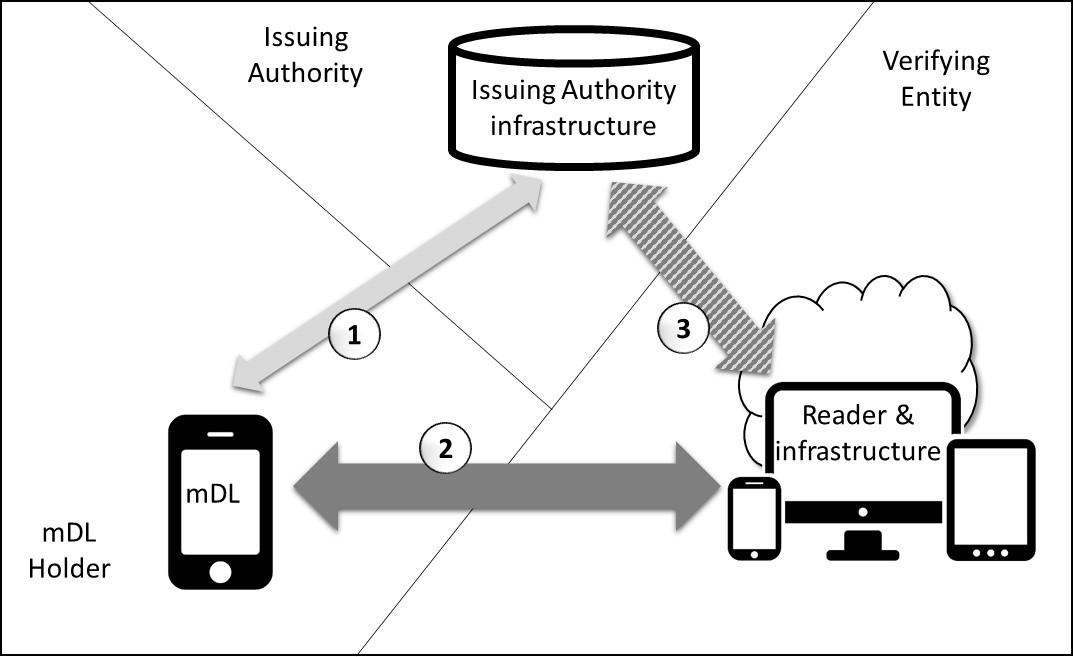
\includegraphics[width=0.8\textwidth]{images/interfaces.png}
	\caption{Ecossistema mDL, incluindo interfaces associadas}
	\label{fig:interfaces}
\end{figure}

% TODO: MAFALDA - REVER e RESUMIR

% O que cada parte trata, de forma geral.
% O qua a parte 5 trata de forma específica (o que é, objetivos, interfaces que trata, ...)

\section{Requisitos}

Os requisitos funcionais abrangidos por esta parte do \textit{standard} para a solução do mDL incluem:

\begin{itemize}
	\item Capaz de funcionar durante verificação num ambiente \textit{offline} (leitor mDL \textit{offline} e mDL \textit{offline}).
	\item Capaz de funcionar durante verificação num ambiente \textit{online} (leitor mDL \textit{online} e mDL \textit{online}).
	\item Inclui mecanismos ou envolve uma arquitetura que permite a partes interessadas na mDL (titular, aplicador da lei ou entidade privada) estabelecer confiança na informação providenciada pela mDL, isto é, ter garantias de que a mDL foi emitida pela alegada autoridade de emissão e que informação não foi alterada.
	\item Confirmar a ligação entre uma mDL e um titular de mDL.
	\item Transmitir privilégios de condução.
	\item Permitir a leitura de informação entre autoridades emissoras.
	\item Permitir que um titular de mDL autorize a libertação de alguma informação selecionada da mDL para um leitor de mDL.
\end{itemize}

Para além destes requisitos, existem ainda alguns problemas que as autoridades de emissão deverão resolver, mas que não são abrangidos por esta versão do ISO/IEC 18013-5:

\begin{itemize}
	\item Mecanismos e tecnologias de armazenamento dos dados da mDL.
	\item Suporte a aplicações de gestão remota da mDL, pelo titular.
	\item Referência ao consentimento do utilizador para um titular de mDL controlar interações online com os sistemas da autoridade de emissão.
\end{itemize}

Existem ainda requisitos técnicos relativos à interface entre uma mDL e um leitor de mDL, que são especificados nesta parte do ISO/IEC 18013:

\begin{itemize}
	\item Estrutura de dados lógicos com as informações da mDL, quando transferidas entre uma mDL e um leitor mDL, deve respeitar os seguintes aspetos:
	\begin{itemize}
		\item Elementos de dados considerados no ISO/IEC 18013-2:
		\begin{itemize}
			\item TODO: ISO/IEC 18013-2
		\end{itemize}

		\item Elementos de dados adicionais:
		\begin{itemize}
			\item Inclusão obrigatória da imagem facial do titular.
			\item Elementos de dados adicionais para "Informação Atualizada".
			\item Identificador adicional que indica o fator de forma.
			\item Grupos de dados mDL, utilizados para transferência de informação seletiva (inclui novos elementos de dados).
		\end{itemize}
	\end{itemize}

	\item Protocolo de comunicação para troca de dados mDL entre uma mDL e um leitor:
	\begin{itemize}
		\item Camada de transmissão:
		\begin{itemize}
			\item ISO/IEC 14443 e/ou ISO/IEC 18092 (NFC)
			\item Interface visual (câmara)
			\item Wi-Fi \textit{Aware}
			\item Internet
			\item \textit{Bluetooth Low Energy} (BLE)
		\end{itemize}
		\item Camada de apresentação:
		\begin{itemize}
			\item Comandos ISO/IEC 7816-4 e ISO/IEC 7816-8 (TODO: Part 2 and Part 3 of this standard) para o equivalente a \textit{Standard Encoding} para mDL
			\item Códigos de barras 2D (para estabelecimento de conexão entre dispositivos e o equivalente a \textit{Compact Encoding} para mDL, na transferência de dados da mDL)
		\end{itemize}
	\end{itemize}

	\item Mecanismos de proteção de dados para serem aplicados, tendo em conta o ISO/IEC 18013-3 - preservar confidencialidade, integridade e autenticação de dados mDL.
\end{itemize}

Especificam-se ainda alguns requisitos funcionais relativos a uma aplicação de leitores de mDL, para assegurar a verificação fiável de uma mDL:

\begin{itemize}
	\item Disponibilidade de verificação de dados (com certificados digitais, por exemplo) de autoridades emissoras, incluindo a definição do modelo de confiança utilizado para uma mDL.
	\item Sequência de leitura para dados de uma mDL.
	\item Sequência de verificação para dados de uma mDL.
\end{itemize}

% TODO: AFONSO - REVER, RESUMIR, MELHORAR

\section{Estrutura de Dados Lógica}

% TODO: DANIEL

\section{Transferência de Dados da mDL}

% TODO: MAFALDA

\section{Mecanismos de Proteção de Dados da mDL}

% TODO: AFONSO

% Identificar os vários algoritmos, primitivas criptográficas e workflows que garantem a segurança da mDL

\section{Implementação da mDL (ISO \textit{compliant})}

% Utilizando bibliotecas open-source, “construir” a mDL de acordo com o ISO (quer no aspeto de segurança como de estrutura de dados)

\section{Conclusões}

% TODO: Conclusões



% TODO: Bibliografia

\end{document}